\section{Generalization \& Regularization}
\textbf{Generalization:} Ein möglichst ''generelles'' Model finden welches möglichst für alle Inputs gültig ist (nicht nur für die Trainingsdaten). Also möglichst gutes Modell aber ohne Overfitting. Somit ein Tradeoff zwischen Variance\&Bias. \\  
\textbf{Regularization:} Eine Methode um die Komplexität des Modells gering zu halten. Ziel ist es, ein einfacheres oder ein möglichst einfaches Modell zu erhalten. Führt zu einer optimalen Balance zwischen Bias\&Variance. Dies wird mit einem Penalty für Komplexität erreicht.
\subsection{Overfitting}
\begin{itemize}
    \item A model that perfectly fits the data does not have to be perfect
    \item In-Sample Error (Trainig error) was minimized (MSE = 0)
    \item Out-of-sample Error (Generalization Error, Test Error) is the MSE of new Data
    \item A good model has a low Generalization Error
    \item Overfitting happens if the MSE of Training Error is small thanks to a complex model but the Generalization Error is large
    \item (too) complex model (many free parameters)
    \item small bias but high variance
\end{itemize}
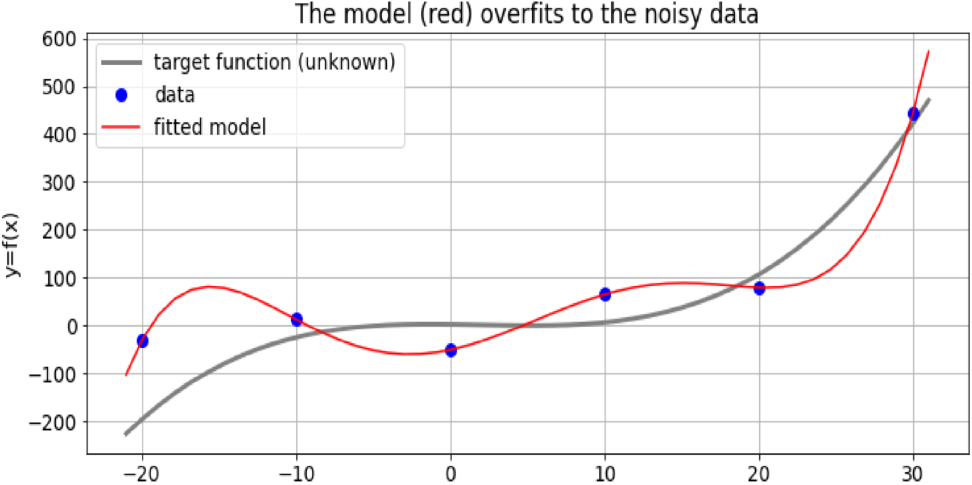
\includegraphics[width=0.9\linewidth]{./img/overfitting.png}

\subsection{Underfitting}
\begin{itemize}
    \item Using a too simple model
    \item In-Sample Error is large
    \item Generalization Error is large
    \item high bias and low variance
\end{itemize}

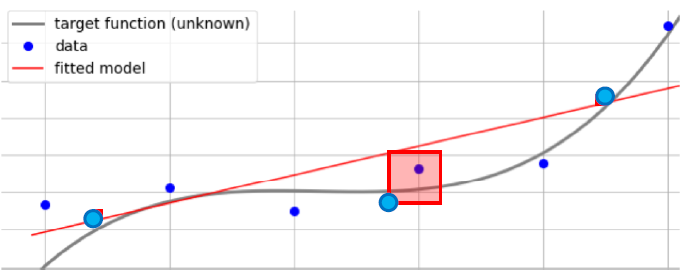
\includegraphics[width=0.9\linewidth]{./img/underfitting.png}

\subsection{Training-Set, Test-Set, Model Evaluation}
\CHECK{TE Titel besser 'Generalization Error'?}
\begin{itemize}
    \item Generalization Error: Der Fehler, den das Modell mit neuen (ungesehenen) Daten erziehlt.
    \item can't be calculated, but estimated (see Test-Error)
    \item Split the data into 2 sets: Training-Set (~80\% of data) \& Test-Set (~20\% of data)
\end{itemize}
\textbf{Training:} 
\begin{itemize}
    \item Fit the model to the training set. This minimizes the \textbf{in-sample error}
\end{itemize} 
\textbf{Evaluating:}
\begin{itemize}
    \item Using the Test-Set produces the \textbf{Test-Error (aka out-of-sample-error)}
    \item This is an estimate of the Generalization Error!
\end{itemize}

\subsection{Bias-Variance Trade-off}
\textbf{Variance (Streuung):} Difference of fits between data sets. Wie hoch ist die Streuung/Abweichung mit neuen Daten. Genauer: Wie gross ist der Unterschied bei verschiedenen Testsets (ungesehenen Daten)? Wenn die alle ''gleich gut/schlecht'' performen ist die Variance klein=besser. (Wie gut spielt also keine Rolle, nur wie gross die Unterschiede sind!). High Variance $\rightarrow$ Overfitting  

\textbf{Bias (Verzerrung):} Results that are systematically prejudiced due to faulty assumptions. Wie gut matcht mein Modell das ''echte Modell'' (Wirklichkeit)? High Bias $\rightarrow$ Modell zu einfach.

\textbf{High Bias}
\begin{itemize}
    \item A too simple model for the given data
\end{itemize}
\textbf{Low Variance}
\begin{itemize}
    \item The model is relatively stable
    \item Very simular model if trained with new data
\end{itemize}
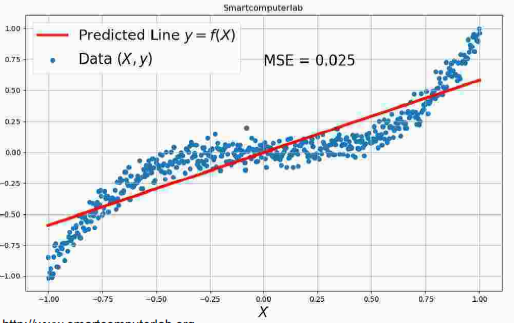
\includegraphics[width=0.6\linewidth]{./img/bias_variance.png}\\
\textbf{Low Bias}
\begin{itemize}
    \item A more complex model can better explain the data
\end{itemize}
\textbf{High Variance}
\begin{itemize}
    \item Given a new datapoint, the MSE can be very large
    \item For a different set with more datapoints, the model may be very different
\end{itemize}
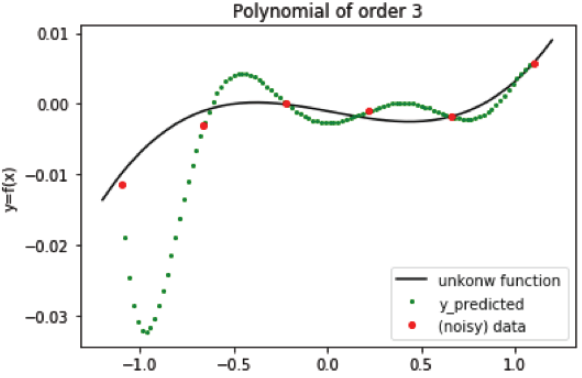
\includegraphics[width=0.6\linewidth]{./img/bias_variance2.png}

\subsubsection{Trade-off}
\begin{itemize}
    \item Higher bias implies lower variance
    \item Lower bias implies higher variance
    \item In practice, all we want is low variance
    \item The model can only be as complex as the data permits
    \item You have to find an optimal balance between bias and variance
\end{itemize}
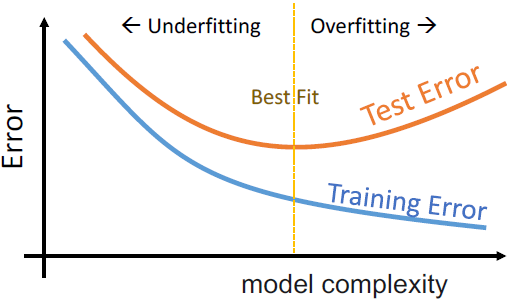
\includegraphics[width=0.6\linewidth]{./img/tradeoff.png}

\subsection{Regularization}
Geht immer um die freien Parameter des Modells. Man bestraft diese. 
\begin{itemize}
    \item Je einfacher das Modell, desto schlechter die Erklärung/ je komplexer das Modell, desto besser die Erklärung
    \item Technique to control the model complexity
    \begin{itemize}
        \item Add a penalty term to the Loss
        \item More complex models get a higher penalty
        \item when 2 models are equal $\rightarrow$ choose the simpler one (Occoams Razor)
        \item Add a constrain to the optimization process
        \item \textit{regularized loss} = \textit{MSE + $\lambda$ model-complexity}
    \end{itemize}
\end{itemize}
\begin{center}
    $\displaystyle\sum_{i = 1}^{n} (y_i - \displaystyle\sum_{j = 1}^{p} x_{ij}\beta_j)^2 + \lambda \displaystyle\sum_{j = 1}^{p}\beta_j^2$
\end{center}
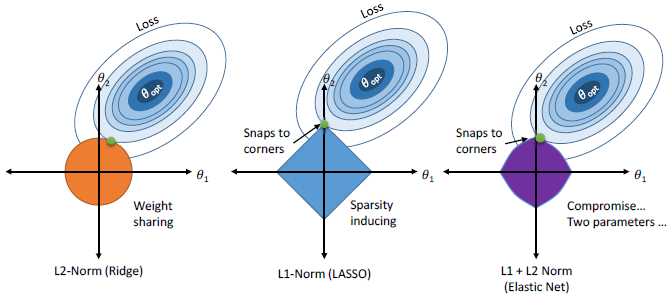
\includegraphics[width=1\linewidth]{./img/regularization.png}

\subsubsection{L1 Regularization}
\begin{itemize}
    \item Absolute Value
    \item Lasso Regression
    \item $mse = \frac{1}{n}\sum_{i=1}^{n} (y_i - h_{\theta}(x_i))^2+\textcolor{red}{\lambda \displaystyle\sum_{i=1}^n|\theta_i|}$
\end{itemize}

\subsubsection{L2 Regularization}
\begin{itemize}
    \item Quadriertes $\theta$
    \item Ridge Regression
    \item $mse = \frac{1}{n}\sum_{i=1}^{n} (y_i - h_{\theta}(x_i))^2+\textcolor{red}{\lambda \displaystyle\sum_{i=1}^n\theta_i^2}$
\end{itemize}

\subsubsection{L1 vs. L2 Regularization}
\begin{itemize}
    \item L1-Regularisierung versucht den Median der Daten zu schätzen
    \item L2-Regularisierung versucht den Mittelwert der Daten zu schätzen, um ein Overfitting zu vermeiden
    \item L1/L2-Norm bestrafen die Modellkomplexität
    \item $\lambda$ legt Verhältnis zwischen Bestrafung und Loss-Function fest
    \begin{itemize}
        \item $\lambda$ = 0 $\rightarrow$ nur Loss-Function relevant ("Bestrafung" = 0)
    \end{itemize}
    \item Entweder einfaches Modell oder komplexeres Modell nehmen und dieses via Generalisierung/ Optimization bestrafen
    \begin{itemize}
        \item zu Beginn gewähltes Modell ist fix/ starr
        \item Mit Generalisierung/ Regluarisierung kann dieses trotzdem nachträglich no "getuned" werden
    \end{itemize}

\end{itemize}


\subsection{Optimization with Keras / Tensorflow}
\begin{minted}{python}
    import tensorflow as tf
    from tensorflow import keras
    from tensorflow.keras import layers
    from tensorflow.keras import regularizers
    model = tf.keras.models.Sequential()
    # define the input. we provide the dimensionality of the input: poly_order
    inputs = keras.Input(shape=(poly_order_MODEL,))
    model.add(inputs)
    output_layer = layers.Dense(1, activation=None, use_bias=True, kernel_regularizer=regularizers.l2(0.005))
    model.add(output_layer)
    # Optimizer
    model.compile(optimizer=keras.optimizers.Adam(learning_rate=0.04),
    loss=keras.losses.MSE, # loss function to minimize
    metrics=[keras.metrics.MSE]) # list of metrics to monitor
\end{minted}

\TODO{Beispiel aus Übung week8\_regularization 'Define a neural network using Keras'}